The empirical results presented in Chapter~\ref{ch:results} establish a clear tension at the
heart of LLM explainability for lay users. Chain-of-Thought prompting emerged as the most
preferred explanation method, receiving the highest number of first-place helpfulness rankings
($n = 45$), yet simultaneously produced, together with Confidence Indication, the lowest median trust scores ($\text{Mdn} = 3.0$)
of all methods tested. Confidence indication ranked a close second in perceived helpfulness
($n = 43$ first-place votes) while also yielding a median trust score of 3.0. SHAP, despite
producing intermediate trust scores, was ranked least helpful by the majority of participants,
consistent with prior literature on the inaccessibility of feature-importance visualizations to
non-technical audiences \cite{chromik_i_2021, kaur_interpreting_2020}.

These findings point toward a concrete design direction: CoT and confidence indication are
complementary. CoT surfaces the reasoning process in a form users find informative and
engaging, but its transparency can expose errors and inconsistencies that erode trust. Confidence
scores, by contrast, provide a lightweight and immediately interpretable signal about the
reliability of individual steps, without requiring users to evaluate the reasoning themselves.
Combining the two methods targets the central tension in the data: making the model's
reasoning transparent while equipping users with a simple signal to calibrate how much weight
to place on each step.

Before presenting the prototype implementation, this chapter first examines why CoT, despite
its advantages, carries structural limitations that make such a complementary signal necessary.

\section{Chain-of-Thought as a Human-Centred Explanation Method}
\label{sec:cot_research}

As established in Chapter~\ref{ch:theory}, XAI methods for LLMs can be broadly divided into post-hoc, intrinsic, and human-centred categories, with the latter consistently outperforming more formal representations in comprehension and perceived usefulness for non-expert audiences \cite{chromik_i_2021}, a pattern confirmed by the low helpfulness ranking of SHAP in the present study. Within the human-centred
category, Chain-of-Thought prompting has emerged as the dominant paradigm and is the method most widely deployed in production systems, with both ChatGPT and Claude surfacing step-by-step reasoning traces as a transparency mechanism.

An alternative to full CoT is the \emph{top-k} or highlight-based self-explanation, in which the model identifies only the few most important words or phrases. Such LLM-generated self-explanations perform on par with traditional post-hoc methods such as LIME and occlusion saliency on faithfulness metrics, while being far cheaper to produce, since they are generated alongside the prediction itself rather than requiring thousands of additional model queries \cite{huang_can_2023}.

\subsection{The Faithfulness Problem}
\label{sec:faithfulness_problem}

Despite its advantages for lay users, CoT carries a fundamental structural limitation:
\emph{faithfulness}, that is, whether the stated reasoning accurately represents the process
by which the model actually arrived at its answer. This limitation helps illustrate the paradox
observed in the study results, where CoT was simultaneously the most preferred and the
least trust-inducing explanation.

Using a suite of tests for measuring CoT faithfulness by
intervening on the stated reasoning and observing whether the model's final answer changes, reveals a substantial variation across tasks: for some tasks the model changes its
answer more than 60\% of the time when the chain of thought is truncated or corrupted; for
others, the final answer is almost entirely unaffected, suggesting the reasoning is largely
post-hoc. Crucially, they find that \textbf{faithfulness shows inverse scaling with model
size}: on most tasks, larger and more capable models produce \emph{less} faithful reasoning
than smaller ones because more capable models can arrive at a confident answer without
needing to rely on the generated trace.\cite{lanham_measuring_2023}

The faithfulness problem has a deeper dimension beyond post-hoc rationalization.  CoT reasoning can be systematically biased by features of the input, such as the position of an answer option or the presence of a suggestive statement, while the stated reasoning provides a different explanation that does not reference the actual cause of the answer shift \cite{turpin_language_2023}. The model therefore produces a plausible-sounding but misleading account of its behaviour.
This concern is compounded by findings on dishonesty in alignment: LLMs trained with RLHF learn to produce responses whose internal representations score low on honesty metrics, particularly in the initial tokens of a refusal or safety response, suggesting that output text can diverge from the model's internal state even during normal operation \cite{huang_dishonesty_2024}.

A related issue concerns the granularity of LLM-generated attributions. When ChatGPT assigns importance scores to individual words, the values cluster on a few rounded levels rather than exhibiting the fine-grained variation produced by traditional methods. This might be due to alignment: the model produces saliency values
plausible for a human to generate, even though a human would not be able to introspect at that level of granularity. This may constitute a faithfulness and understandability trade-off, where the explanation is more accessible but less precisely tied to the model's computation \cite{huang_can_2023}.

These considerations together characterize CoT as a high-information, trust-calibrating explanation type that is, however, structurally prone to unfaithfulness, particularly in larger models and on tasks where the model can answer confidently without explicit reasoning. The paradox identified in the present data,
namely that CoT is simultaneously the most preferred and the least trust-inducing explanation, may therefore reflect an empirically appropriate response by participants: transparency about a reasoning process that contains errors or inconsistencies reduces trust, even if that reasoning is not a faithful account of what the model actually did.

\subsection{Technically-Grounded Alternatives}

More technically ambitious approaches attempt to ground explanations in the model's internal representations rather than its output text, operating directly on hidden embeddings at intermediate layers and in principle providing explanations causally connected to the model's computation. Such methods are not subject to the same faithfulness failures as CoT, but they are substantially less interpretable by non-expert users, limiting their deployment potential in the human-centred XAI contexts examined here.

A notable example is \textbf{SelfIE} \cite{chen_selfie_2024}, which enables LLMs to interpret their own hidden embeddings via a secondary forward pass, producing explanations structurally grounded in internal representations rather than output text. However, SelfIE requires white-box access to model weights, operates at a layer-level granularity opaque to non-technical users, and has so far been evaluated primarily on a single model family, leaving its broader generalisability open.

An alternative strand of research has explored \textbf{neural template} generation as a human-interpretable explanation mechanism for AI systems. NETE (Neural Template Explanations), is a framework originally developed for explainable recommender systems that bridges template-based and free-form natural language generation. Rather than relying on manually predefined sentence templates, which constrain expressiveness and cannot adapt to item-specific features, NETE learns \emph{neural templates} from data via a novel Gated Fusion Recurrent Unit (GFRU). The GFRU runs two parallel GRU decoders: a \emph{context GRU} that generates the surrounding sentence structure, and a \emph{feature GRU} that inserts a specified item feature at the appropriate position; a gated fusion unit then combines their outputs at each decoding step. This architecture allows the system to generate targeted, controllable explanations such as \emph{``The ramen was delicious''} when given the feature \emph{ramen}, closely matching ground-truth user reviews. Empirically, NETE produces substantially more unique and feature-diverse explanations than prior neural generation baselines (Att2Seq, NRT), with improvements exceeding 100\% on BLEU-4 and ROUGE-2 n-gram metrics across hotel, restaurant, and movie review datasets.\cite{li_generate_2020}

However, the neural template paradigm carries several limitations that constrain its transferability to general-purpose LLM explainability. First, NETE requires structured training data in which each user-item interaction is paired with both a ground-truth feature label and a reference explanation sentence, a requirement that is not met in most LLM deployment settings. Second, the GFRU architecture is task-specific: it is designed to slot a single feature word into a recommendation-oriented sentence template, and does not straightforwardly generalize to the open-ended reasoning traces or multistep factual answers that characterize LLM outputs. Third, like CoT, the generated text remains an output-level artefact and carries no guarantee of faithfulness to the model's internal computation; the template constrains surface form but not the accuracy of the underlying reasoning.

\subsection{The Design Gap and the Prototype Direction}

The survey findings and the literature review together point toward a design space that
remains substantially unoccupied: explanation methods grounded enough in model internals
to be reliable, as SelfIE aims to be, yet rendered in forms accessible to lay users, as neural
templates and CoT attempt to achieve. SelfIE's white-box requirements and layer-level
granularity place it out of reach for the deployment contexts studied here, while NETE's
task-specific architecture cannot be applied to open-ended LLM reasoning.

The most practically viable path, given the constraints of both technical feasibility and lay
usability, is to augment CoT with a complementary signal that allows users to calibrate their
reliance on the stated reasoning without requiring any knowledge of model architecture. The
study results suggest that confidence scores are precisely such a signal: they were ranked
second in perceived helpfulness, are derivable directly from the model's token-level
log-probabilities, and communicate uncertainty in a form that requires no technical
interpretation. The prototype described in the following section operationalizes this
combination.

\section{Prototype Implementation}
\label{sec:prototype}
 
Building on the findings of the user study, a prototype was developed that combines
Chain-of-Thought reasoning with per-step confidence scores (CoT\,+\,CONF). This pairing
is motivated by the complementary properties of the two methods identified in the study:
CoT functions as a high-information, trust-calibrating explanation that surfaces reasoning
steps the user can evaluate, while confidence scores provide a lightweight signal that
allows users to assess the reliability of each step without requiring technical knowledge
of model architecture. Together, they target the central tension identified in the results:
making the model's reasoning transparent while keeping it simple to understand for lay-users.
 
\subsection{Design Rationale}
 
The prototype moves away from a forced JSON output format used in the survey app (Section~\ref{sec:stimulusGeneration}) of CoT extraction, which proved brittle and difficult to parse consistently. Instead, steps are structured as a simpler, delimited sequence, which is both easier for the model to produce reliably and of similar ease to parse programmatically. Each reasoning step is assigned an
average confidence score, derived from the token-level log-probabilities returned by the
underlying language model. Steps whose mean confidence falls below a user-configurable
threshold are automatically regenerated; users may also trigger manual regeneration of
any individual step. In the frontend, steps are colour-coded on a red-to-green scale
reflecting their confidence, giving users an immediate visual summary of where the model
is uncertain.
 
\subsection{Architecture Overview}
 
The application follows a modular FastAPI architecture. Source code and setup instructions
are available in the project repository: \url{https://github.com/rieselin/BA_XAI_for_LLMs}

The top-level directory structure is as follows:
 
\begin{lstlisting}
src/
  api/
    routes.py              # FastAPI endpoints
  core/
    model_loader.py        # get_model()
    prompt_builder.py      # all prompt templates
    generation.py          # unified generation logic
  reasoning/
    cot.py                 # CoT extraction/parsing
    confidence.py          # token probability logic
    pipeline.py            # orchestrator
  schemas/
    request.py             # Request models
    response.py            # Response models
  index.html               # Frontend
  main.py                  # FastAPI app setup
\end{lstlisting}
 
\subsection{Class Structure}
 
The system's data model and processing classes are described below. Figure~\ref{fig:class_classes}
shows the schema and request/response classes, while Figure~\ref{fig:class_methods} shows
the processing classes together with their methods.
 
\begin{figure}[htbp]
  \centering
  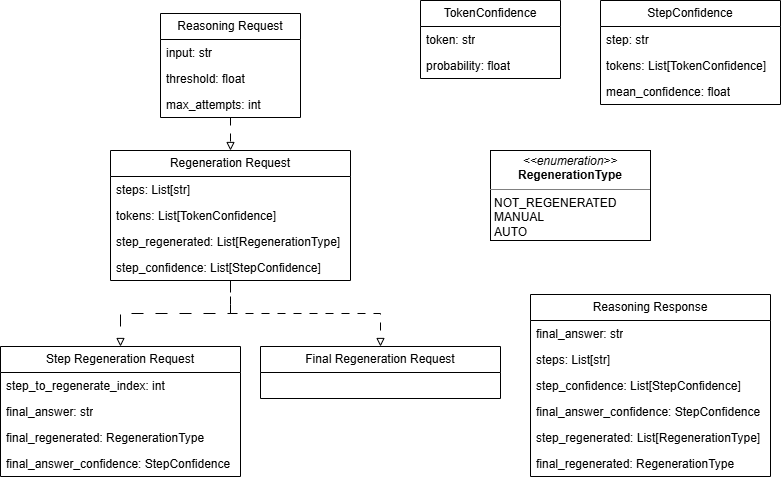
\includegraphics[width=0.9\textwidth]{diagrams/class_diagram_classes.png}
  \caption{Class diagram showing the schema and data-model classes}
  \label{fig:class_classes}
\end{figure}
 
\begin{figure}[htbp]
  \centering
  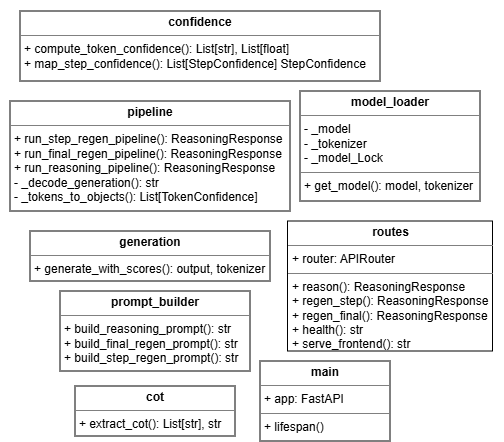
\includegraphics[width=0.7\textwidth]{diagrams/class_diagram_methods.png}
  \caption{Class diagram showing the processing classes with their methods.}
  \label{fig:class_methods}
\end{figure}
 
\subsubsection{Data and Schema Classes}

The request pipeline begins with a \localtt{ReasoningRequest}, which carries the user's
input string, a confidence threshold, and a maximum number of regeneration
attempts. A \localtt{ReasoningRequest} is extended by \localtt{RegenerationRequest}, which
additionally holds the list of reasoning steps, the token-level confidence data for each
step (\localtt{List[TokenConfidence]}), the regeneration status of each step
(\localtt{List[Regeneration-Type]}), and the aggregated per-step confidence objects
(\localtt{List[StepConfidence]}).
 
Two specialisations of \localtt{RegenerationRequest} exist. A
\localtt{StepRegenerationRequest} is used when a single step must be re-generated: it adds
the index of the step to regenerate, the current final answer, the regeneration type of
the final answer, and its confidence. A \localtt{FinalRegenerationRequest} carries the
same fields minus the step index, and is used when only the concluding answer requires
regeneration.
 
The \localtt{ReasoningResponse} returned to the client contains the final answer string,
the list of reasoning steps, per-step confidence objects, the confidence of the final
answer (\localtt{StepConfidence}), and the regeneration status of every step and of the
final answer.
 
Two auxiliary value types support the confidence representation. A
\localtt{TokenConfidence} pairs a decoded token string with its probability. A
\localtt{StepConfidence} groups an entire reasoning step with its token list and the
mean confidence across those tokens. Finally, \localtt{RegenerationType} is an enumeration
with three values: \localtt{NOT\_REGENERATED}, \localtt{MANUAL}, and \localtt{AUTO},
recording how each step was produced.
 
\subsubsection{Processing Classes}
 
The \localtt{model\_loader} module maintains a singleton model and tokenizer
(\localtt{\_model}, \localtt{\_tokenizer}) together with an async lock (\localtt{\_model\_Lock})
and exposes a single \localtt{get\_model()} method that returns both objects.
 
Prompt construction is centralised in the \localtt{prompt\_builder}, which provides three
template methods: \localtt{build\_reasoning\_prompt()} for the initial CoT query,
\localtt{build\_step\_regen\_prompt()} for single-step regeneration, and
\localtt{build\_final\_regen\_prompt()} for regenerating the concluding answer.
 
The \localtt{generation} class wraps the low-level inference call in a single method,
\localtt{generate\_with\_scores()}, which returns the raw output tokens together with the
tokenizer, making log-proba\-bi\-li\-ty extraction straightforward for downstream modules.
 
Confidence computation is handled by two methods on the \localtt{confidence} class.
\localtt{compute\_token\_confidence()} accepts the raw output and tokenizer and returns a
parallel list of decoded token strings and their probabilities. \localtt{map\_step\_confidence()}
maps these token-level values onto the step boundaries identified by the CoT parser,
returning a list of \localtt{StepConfidence} objects.
 
The \localtt{cot} module exposes a single method, \localtt{extract\_cot()}, which parses
the model output into a list of step strings and the final answer string.
 
Endpoint routing is provided by \localtt{routes} (registered as an
\localtt{APIRouter}), which exposes four HTTP handlers: \localtt{reason()} for the primary
inference request, \localtt{regen\_step()} and \localtt{regen\_final()} for targeted
regeneration, \localtt{health()} for a liveness probe, and \localtt{serve\_frontend()} to
serve the single-page HTML interface.
 
The \localtt{pipeline} class is the central orchestrator. Its public entry point,
\localtt{run\_reasoning\_pipeline()}, coordinates all other modules and calls the two
regeneration sub-pipelines internally whenever automatic regeneration is triggered.
\localtt{run\_step\_regen\_pipeline()} and \localtt{run\_final\_regen\_pipeline()} therefore
serve a dual role: they are invoked by \localtt{run\_reasoning\_pipeline()} during the
automatic threshold check, and are also called directly by the \localtt{regen\_step()} and
\localtt{regen\_final()} route handlers when the user requests manual regeneration from the
frontend. Two private utilities, \localtt{\_decode\_generation()} and
\localtt{\_tokens\_to\_objects()}, handle token decoding and the conversion of raw
probability arrays into \localtt{TokenConfidence} objects respectively. All three pipeline
methods return a \localtt{ReasoningResponse}.
 
The entry point \localtt{main.py} instantiates the FastAPI \localtt{app} and registers a
\localtt{lifespan()} context manager that triggers the asynchronous model load on startup.
 
\subsection{Application Flow}
 
On startup, the application executes an asynchronous \localtt{get\_model()} call and waits
until the model and tokenizer are resident in memory before accepting requests. The
primary inference route (\localtt{/reason}) accepts a \localtt{ReasoningRequest} and
delegates to \localtt{run\_reasoning\_pipeline()}, which proceeds as follows:
 
\begin{enumerate}
  \item \textbf{Prompt construction.} \localtt{build\_reasoning\_prompt()} formats the user
        query into a CoT prompt.
  \item \textbf{Generation.} \localtt{generate\_with\_scores()} calls the model and returns
        output tokens with log-probabilities.
  \item \textbf{Decoding.} \localtt{\_decode\_generation()} converts raw token ids to
        strings; \localtt{compute\_token\_confidence()} extracts per-token probabilities.
  \item \textbf{Parsing.} \localtt{extract\_cot()} segments the decoded output into
        individual reasoning steps and the final answer.
  \item \textbf{Confidence mapping.} \localtt{map\_step\_confidence()} aligns token
        probabilities with step boundaries to produce \localtt{StepConfidence} objects.
  \item \textbf{Threshold check.} Any step whose mean confidence falls below the
        user-supplied threshold is queued for automatic regeneration. Steps above the
        threshold are retained as-is.
  \item \textbf{Regeneration (if required).} Steps flagged in the previous phase are
        passed individually to \localtt{run\_step\_regen\_pipeline()}, which calls
        \localtt{build\_step\_regen\_prompt()}, reruns generation and confidence mapping,
        and marks the step as \localtt{AUTO}. If the final answer is below the threshold,
        \localtt{run\_final\_regen\_pipeline()} is invoked analogously using
        \localtt{build\_final\_regen\_prompt()}.
  \item \textbf{Response assembly.} A \localtt{ReasoningResponse} is constructed from the
        (potentially updated) steps, confidence objects, and regeneration status flags, and
        returned to the client.
\end{enumerate}
 
The same sub-pipelines are also reachable directly from the frontend: when the user
manually requests regeneration of a step or of the final answer via a call to
\localtt{/reason/step} or \localtt{/reason/final} the route handler calls
\localtt{run\_step\_regen\_pipeline()} or \localtt{run\_final\_regen\_pipeline()}
depending on which endpoint was invoked, following the same logic as the automatic path but recording the regeneration type as \localtt{MANUAL} rather than \localtt{AUTO}. The frontend displays
each step with a colour gradient from red
(low confidence) to green (high confidence), and exposes the regeneration threshold as a
configurable input, allowing users to adjust the sensitivity of automatic regeneration to
their needs.
 
For full setup instructions of both this prototype and the survey demo app see the project \href{https://github.com/rieselin/BA_XAI_for_LLMs/blob/main/README.md}{\underline{README}}\footnote{\url{https://github.com/rieselin/BA_XAI_for_LLMs/blob/main/README.md}}.